\subsection{Referenční popis obrázku}
Jako první byl implementován systém pro práci s referenčním popisem obrázku.
Aby bylo možné vytvořenou implementaci rovnou testovat, bylo nutné zvolit nějaký konkrétní obrázek,
na kterém by bylo možné jednotlivé části zkoušet.
Pro tento účel byla zvolena kresba
\todo{doplnit odkud obrázek je + správě ozdrojovat},
která je zobrazena na Obrázku~\ref{fig:summer}.
\todo{doplnit nebo odebrat bílý okraj obrázku}

\begin{figure}[ht!]
	\centering
	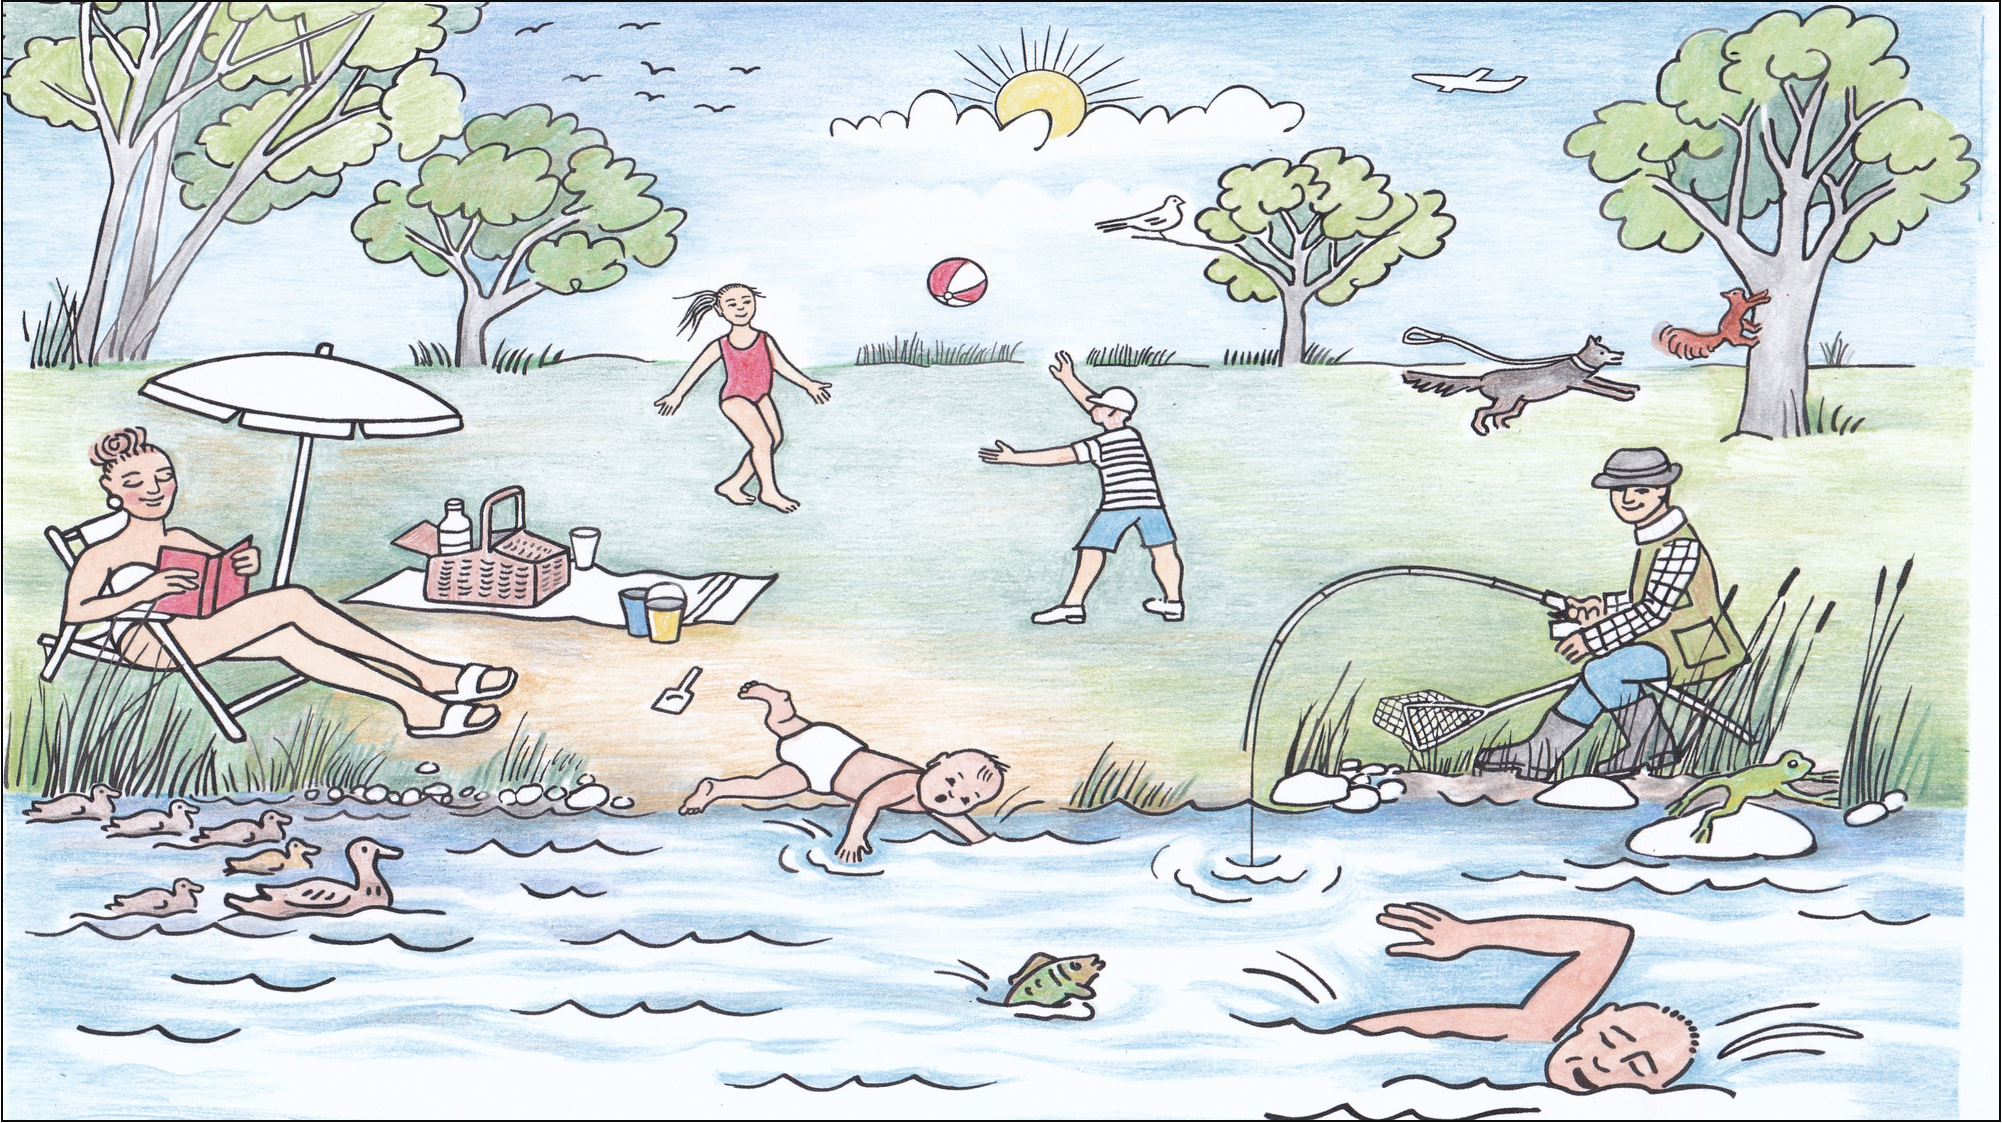
\includegraphics[width=\textwidth]{./src/imgs/summer.png}
	\caption{Kresba použitá při implementaci pro testování}\label{fig:summer}
\end{figure}

Jak bylo definováno v kapitole~\ref{subsec:reprezentace_znalosti}, referenční popis obrázku se skládá z
množiny objektů, jejich atributů a vazeb mezi nimi.
Nyní bylo potřeba stanovit nějaký datový formát, který by umožnil tuto strukturu dobře zachytit.

\newpage
Základním prvkem referenčního popisu je struktura \enquote{\texttt{Scene}}, která obsahuje informace o obrázku, objekty s atributy a vazby mezi nimi.

Objekty byly definované strukturou \enquote{\texttt{SceneObject}}, která popisuje objekt ve scéně a jeho atributy.
Každý \texttt{SceneObject} obsahuje informaci o svém názvu, umístění, velikosti a hierarchii vůči ostatním objektům.
Dále si každý \texttt{SceneObject} udržuje list atributů a tagů, které mu byly expertem přiděleny.

Další strukturou, která byla definována jako součást referenčního popisu, je \enquote{\texttt{Triplet}}.
Tato struktura slouží k popisu vazeb mezi objekty, obsahuje názvy dvou objektů a k nim název vazby.

Schéma implementovaných struktur a jejich provázání je na Obrázku~\ref{fig:schema_impl_ref_popis}.
Zdrojový kód je pak možné si prohlédnout
\todo{doplnit odkaz na zdrojáky}
\todo{vyměnit tabulky za pseudo-kód?}
\todo{vysvětlit u32 a Vec<>?}

% \todo{vyměnit za tabulku? Nechat jako Rust kód a obarvit, nebo se tvářit že to je pseudo-kód?}
% \todo{přidat nějaký popisek a označení (listing?)}
% \todo{vysvětlovat zkratky datových typů? Nebo nahradit slovy?}
% 
% \begin{verbatim}
% struct Scene {
%     width: u32,                 // šířka obrázku v pixelech
%     height: u32,                // výška obrázku v pixelech
%     image_path: String,         // cesta na disku k souboru s obrázkem
%     objects: Vec<SceneObject>,  // list objektů ve scéne
%     triplets: Vec<Triplet>,     // list vazeb mezi objekty
% }
% \end{verbatim}

% \begin{verbatim}
% struct SceneObject {
%     name: String,                       // název tohoto objektu
%     tags: Vec<String>,                  // list tagů přiřazených k tomuto objektu
%     top_left_corner: (u32, u32),        // pozice levého horního okraje bounding-boxu
%     size: (u32, u32),                   // velikost objektu v pixelech ve formátu (šířka, výška)
%     parents: Vec<String>,               // list (názvů) objektů, které jsou rodiče tohoto objektu
%     children: Vec<String>,              // list (názvů) objektů, které jsou potomci tohoto objektu
%     attributes: Vec<(String, String)>,  // list atributů jako dvojic "(název, hodnota)"
% }
% \end{verbatim}

% \begin{verbatim}
% pub struct Triplet {
%     pub from: String,       // název zdrojového objektu
%     pub predicate: String,  // název vazby
%     pub to: String,         // název cílového objektu
% }
% \end{verbatim}
\begin{figure}[ht!]
	\centering
	\begin{tikzpicture}
		\node[inner sep=0] (ref) at (0, 0) {
			\begin{tabular}{|l|l|l|}
				\hline
				\multicolumn{2}{|c|}{\large \texttt{Scene}}                    \\
				\hline
				\textbf{\textit{Pole}} & \textbf{\textit{Datový typ}}          \\
				\hline
				\texttt{width}         & \texttt{u32}                          \\
				\texttt{height}        & \texttt{u32}                          \\
				\texttt{image\_path}   & \texttt{String}                       \\
				\texttt{objects}       & \texttt{Vec<\phantom{ SceneObject }>} \\
				\texttt{triplets}      & \texttt{Vec<\phantom{ Triplet }>}     \\
				\hline
			\end{tabular}
		};
		\node[anchor=north, inner sep=1pt] (trip) at ($(ref.south) + (0, -1)$) {
			\begin{tabular}{|l|l|l|}
				\hline
				\multicolumn{2}{|c|}{\large \texttt{Triplet}}         \\
				\hline
				\textbf{\textit{Pole}} & \textbf{\textit{Datový typ}} \\
				\hline
				\texttt{from}          & \texttt{String}              \\
				\texttt{predicate}     & \texttt{String}              \\
				\texttt{to}            & \texttt{String}              \\
				\hline
			\end{tabular}
		};
		% \node[anchor=south west, inner sep=1pt] (so) at ($(trip.south east) + (2.0, 0)$) {
		\node[anchor=south west, inner sep=1pt] (so) at ($(ref.east|-trip.south) + (1, 0)$) {
			\begin{tabular}{|l|l|l|}
				\hline
				\multicolumn{2}{|c|}{\large \texttt{SceneObject}}           \\
				\hline
				\textbf{\textit{Pole}}     & \textbf{\textit{Datový typ}}   \\
				\hline
				\texttt{name}              & \texttt{String}                \\
				\texttt{tags}              & \texttt{Vec<String>}           \\
				\texttt{top\_left\_corner} & \texttt{(u32, u32)}            \\
				\texttt{size}              & \texttt{(u32, u32)}            \\
				\texttt{parents}           & \texttt{Vec<String>}           \\
				\texttt{children}          & \texttt{Vec<String>}           \\
				\texttt{attributes}        & \texttt{Vec<(String, String)>} \\
				\hline
			\end{tabular}
		};
		\node[anchor=south east] (trmark) at ($(ref.south east) + (-32pt, 0)$) {\texttt{Triplet}};
		\node[anchor=south east] (somark) at ($(ref.south east) + (-12pt, \baselineskip)$) {\texttt{SceneObject}};
		\node[draw=blue, rounded corners=2mm, inner sep=3pt] (trborder) at ($(trmark) + (0, 0.5pt)$) {\texttt{\phantom{Triplet}}};
		\node[draw=blue, rounded corners=2mm, inner sep=3pt] (soborder) at ($(somark) + (0, 0.5pt)$) {\texttt{\phantom{SceneObject}}};
		\draw[blue, -Stealth] (trborder.south) to (trmark|-trip.north);
		\draw[blue, rounded corners=2mm, -Stealth] (soborder.north) -- ++(0, 1.0) -| (so.north);
		% \draw[blue, rounded corners=2mm, -Stealth] (soborder.north) |- ($(0, 0.2) + (so.west)$);
	\end{tikzpicture}
	\caption{Schéma implementace referenčního popisu}\label{fig:schema_impl_ref_popis}
\end{figure}

Ve struktuře \texttt{Scene} je význam jednotlivých polí poměrně jednoduchý.
Pole \texttt{width} a \texttt{height} vyjadřují výšku a šířku obrázku v pixelech, \texttt{image\_path} udává cestu k souboru, který obsahuje samotný obrázek.
Pole \texttt{objects} a \texttt{triplets} pak obsahují list objektů a tripletů.

Struktura \texttt{Triplet} je velmi jednoduchá.
Její pole \texttt{from} a \texttt{to} jsou názvy zdrojového, respektive cílového, objektu.
Pole \texttt{predicate} je název samotné vazby mezi těmito objekty.

Poslední struktura \texttt{SceneObject}, která popisuje samotné objekty, je nejsložitější.
Pole \texttt{name} udává název daného objektu, který slouží zároveň jako identifikátor a musí být tudíž unikátní.
Může nastat situace, že v obrázku bude více objektů, které by přirozeně byly označené stejně, například dva stromy.
Pro tento případ byla implementována možnost objekty číslovat a tím tak jednoznačně rozlišit i objekty stejného typu.
Číslování objektů je součástí jejich názvu a má formát \enquote{\texttt{\#n}} kde $n$ je přirozené číslo označující index objektu.
Například \enquote{\texttt{strom \#1}} a \enquote{\texttt{strom \#2}}.

Dvojice polí \texttt{top\_left\_corner} a \texttt{size} udávají velikost a pozici objektu zdrojovém obrázku.
Jedná se o souřadnice levého horního rohu ohraničujícího rámce (bounding-boxu) a velikost tohoto rámce v pixelech.
Obě pole mají jako uvedený datový typ \texttt{(u32, u32)}, který reprezentuje souřadnice $(i, j)$ kde $i,j \in \mathbb{N}^{0}$.
V obrázku je dle konvence jako počátek souřadnic uvažován levý horní roh.
\todo{zdrojovat kde jsem vzal \enquote{konvenci}?}

Pole \texttt{tags} reprezentuje list tagů, které expert obrázku přiřadil.
Jejich účel byl popsán v kapitole~\ref{subsec:hodnoceni}.
Další dvojice polí \texttt{parents} a \texttt{children} pak reprezentuje list objektů, které jsou rodiče, respektive potomci, daného objektu.

Po formální definice formátů a datový typů bylo potřeba určit, jakým způsobem bude expert referenční popis tvořit.
Pro tuto práci bylo rozhodnuto, že tvorba referenčního popisu bude spočívat v napsání strukturovaného textového souboru.
Zvolen byl textový formát \texttt{JSON}, který představuje dobrý kompromis mezi čitelností člověkem a strojovou zpracovatelností.

Ukázka části referenčního popisu je na Listing~\ref{lst:ref_popis_real_example}.
\todo{jak se česky skloňuje a překládá Listing?}
\todo{ukázat stejný popis graficky jako schéma + obrázek?}
\clearpage
% \def\lstlabel{label=}
\begin{lstlisting}[
	% there are many more options of styling, see the official documentation, these are just the defaults I like
	frame=single, % make single-line frame around the verbatim
	framesep=2mm, % put some more spacing between the frame and text
	aboveskip=5mm, % put some more space above the box
	basicstyle={\linespread{0.83}\footnotesize\ttfamily}, % use typewriter (monospace) font
	caption={Příklad jednoduchého referenčního popisu}, % set the caption text
	captionpos=b, % put the caption at the bottom (b) or top (t) or both (bt)
	label={lst:ref_popis_real_example}, % label to be referenced via \ref{}
	numbers=left, % line numbers on the left
	numberstyle={\scriptsize\ttfamily\color{black!60}}, % the style for line numbers
	escapeinside={<@}{@>} % between those sequences are command evaluated
]
<@\textcolor[HTML]{FF1010}{\texttt{\{}}@>
<@\textcolor[HTML]{000000}{\texttt{\ \ }}@><@\textcolor[HTML]{255CFF}{\texttt{"width"}}@><@\textcolor[HTML]{1041FF}{\texttt{:}}@><@\textcolor[HTML]{000000}{\texttt{\ }}@><@\textcolor[HTML]{DE6F10}{\texttt{2002}}@><@\textcolor[HTML]{1041FF}{\texttt{,}}@>
<@\textcolor[HTML]{000000}{\texttt{\ \ }}@><@\textcolor[HTML]{255CFF}{\texttt{"height"}}@><@\textcolor[HTML]{1041FF}{\texttt{:}}@><@\textcolor[HTML]{000000}{\texttt{\ }}@><@\textcolor[HTML]{DE6F10}{\texttt{1123}}@><@\textcolor[HTML]{1041FF}{\texttt{,}}@>
<@\textcolor[HTML]{000000}{\texttt{\ \ }}@><@\textcolor[HTML]{255CFF}{\texttt{"image\_path"}}@><@\textcolor[HTML]{1041FF}{\texttt{:}}@><@\textcolor[HTML]{000000}{\texttt{\ }}@><@\textcolor[HTML]{418310}{\texttt{"./data/imgs/summer.png"}}@><@\textcolor[HTML]{1041FF}{\texttt{,}}@>
<@\textcolor[HTML]{000000}{\texttt{\ \ }}@><@\textcolor[HTML]{255CFF}{\texttt{"objects"}}@><@\textcolor[HTML]{1041FF}{\texttt{:}}@><@\textcolor[HTML]{000000}{\texttt{\ }}@><@\textcolor[HTML]{FF1010}{\texttt{[}}@>
<@\textcolor[HTML]{000000}{\texttt{\ \ \ \ }}@><@\textcolor[HTML]{FF1010}{\texttt{\{}}@>
<@\textcolor[HTML]{000000}{\texttt{\ \ \ \ \ \ }}@><@\textcolor[HTML]{255CFF}{\texttt{"name"}}@><@\textcolor[HTML]{1041FF}{\texttt{:}}@><@\textcolor[HTML]{000000}{\texttt{\ }}@><@\textcolor[HTML]{418310}{\texttt{"tree\ \#1"}}@><@\textcolor[HTML]{1041FF}{\texttt{,}}@>
<@\textcolor[HTML]{000000}{\texttt{\ \ \ \ \ \ }}@><@\textcolor[HTML]{255CFF}{\texttt{"tags"}}@><@\textcolor[HTML]{1041FF}{\texttt{:}}@><@\textcolor[HTML]{000000}{\texttt{\ }}@><@\textcolor[HTML]{FF1010}{\texttt{[}}@><@\textcolor[HTML]{418310}{\texttt{"environment"}}@><@\textcolor[HTML]{FF1010}{\texttt{]}}@><@\textcolor[HTML]{1041FF}{\texttt{,}}@>
<@\textcolor[HTML]{000000}{\texttt{\ \ \ \ \ \ }}@><@\textcolor[HTML]{255CFF}{\texttt{"top\_left\_corner"}}@><@\textcolor[HTML]{1041FF}{\texttt{:}}@><@\textcolor[HTML]{000000}{\texttt{\ }}@><@\textcolor[HTML]{FF1010}{\texttt{[}}@><@\textcolor[HTML]{DE6F10}{\texttt{1194}}@><@\textcolor[HTML]{1041FF}{\texttt{,}}@><@\textcolor[HTML]{000000}{\texttt{\ }}@><@\textcolor[HTML]{DE6F10}{\texttt{146}}@><@\textcolor[HTML]{FF1010}{\texttt{]}}@><@\textcolor[HTML]{1041FF}{\texttt{,}}@>
<@\textcolor[HTML]{000000}{\texttt{\ \ \ \ \ \ }}@><@\textcolor[HTML]{255CFF}{\texttt{"size"}}@><@\textcolor[HTML]{1041FF}{\texttt{:}}@><@\textcolor[HTML]{000000}{\texttt{\ }}@><@\textcolor[HTML]{FF1010}{\texttt{[}}@><@\textcolor[HTML]{DE6F10}{\texttt{264}}@><@\textcolor[HTML]{1041FF}{\texttt{,}}@><@\textcolor[HTML]{000000}{\texttt{\ }}@><@\textcolor[HTML]{DE6F10}{\texttt{220}}@><@\textcolor[HTML]{FF1010}{\texttt{]}}@><@\textcolor[HTML]{1041FF}{\texttt{,}}@>
<@\textcolor[HTML]{000000}{\texttt{\ \ \ \ \ \ }}@><@\textcolor[HTML]{255CFF}{\texttt{"parents"}}@><@\textcolor[HTML]{1041FF}{\texttt{:}}@><@\textcolor[HTML]{000000}{\texttt{\ }}@><@\textcolor[HTML]{FF1010}{\texttt{[}}@><@\textcolor[HTML]{FF1010}{\texttt{]}}@><@\textcolor[HTML]{1041FF}{\texttt{,}}@>
<@\textcolor[HTML]{000000}{\texttt{\ \ \ \ \ \ }}@><@\textcolor[HTML]{255CFF}{\texttt{"children"}}@><@\textcolor[HTML]{1041FF}{\texttt{:}}@><@\textcolor[HTML]{000000}{\texttt{\ }}@><@\textcolor[HTML]{FF1010}{\texttt{[}}@><@\textcolor[HTML]{418310}{\texttt{"branch"}}@><@\textcolor[HTML]{FF1010}{\texttt{]}}@><@\textcolor[HTML]{1041FF}{\texttt{,}}@>
<@\textcolor[HTML]{000000}{\texttt{\ \ \ \ \ \ }}@><@\textcolor[HTML]{255CFF}{\texttt{"attributes"}}@><@\textcolor[HTML]{1041FF}{\texttt{:}}@><@\textcolor[HTML]{000000}{\texttt{\ }}@><@\textcolor[HTML]{FF1010}{\texttt{[}}@>
<@\textcolor[HTML]{000000}{\texttt{\ \ \ \ \ \ \ \ }}@><@\textcolor[HTML]{FF1010}{\texttt{[}}@><@\textcolor[HTML]{418310}{\texttt{"color"}}@><@\textcolor[HTML]{1041FF}{\texttt{,}}@><@\textcolor[HTML]{000000}{\texttt{\ }}@><@\textcolor[HTML]{418310}{\texttt{"green"}}@><@\textcolor[HTML]{FF1010}{\texttt{]}}@><@\textcolor[HTML]{1041FF}{\texttt{,}}@>
<@\textcolor[HTML]{000000}{\texttt{\ \ \ \ \ \ \ \ }}@><@\textcolor[HTML]{FF1010}{\texttt{[}}@><@\textcolor[HTML]{418310}{\texttt{"color"}}@><@\textcolor[HTML]{1041FF}{\texttt{,}}@><@\textcolor[HTML]{000000}{\texttt{\ }}@><@\textcolor[HTML]{418310}{\texttt{"brown"}}@><@\textcolor[HTML]{FF1010}{\texttt{]}}@>
<@\textcolor[HTML]{000000}{\texttt{\ \ \ \ \ \ }}@><@\textcolor[HTML]{FF1010}{\texttt{]}}@>
<@\textcolor[HTML]{000000}{\texttt{\ \ \ \ }}@><@\textcolor[HTML]{FF1010}{\texttt{\}}}@><@\textcolor[HTML]{1041FF}{\texttt{,}}@> <@\textcolor[HTML]{FF1010}{\texttt{\{}}@>
<@\textcolor[HTML]{000000}{\texttt{\ \ \ \ \ \ }}@><@\textcolor[HTML]{255CFF}{\texttt{"name"}}@><@\textcolor[HTML]{1041FF}{\texttt{:}}@><@\textcolor[HTML]{000000}{\texttt{\ }}@><@\textcolor[HTML]{418310}{\texttt{"bird"}}@><@\textcolor[HTML]{1041FF}{\texttt{,}}@>
<@\textcolor[HTML]{000000}{\texttt{\ \ \ \ \ \ }}@><@\textcolor[HTML]{255CFF}{\texttt{"tags"}}@><@\textcolor[HTML]{1041FF}{\texttt{:}}@><@\textcolor[HTML]{000000}{\texttt{\ }}@><@\textcolor[HTML]{FF1010}{\texttt{[}}@><@\textcolor[HTML]{418310}{\texttt{"animal"}}@><@\textcolor[HTML]{FF1010}{\texttt{]}}@><@\textcolor[HTML]{1041FF}{\texttt{,}}@>
<@\textcolor[HTML]{000000}{\texttt{\ \ \ \ \ \ }}@><@\textcolor[HTML]{255CFF}{\texttt{"top\_left\_corner"}}@><@\textcolor[HTML]{1041FF}{\texttt{:}}@><@\textcolor[HTML]{000000}{\texttt{\ }}@><@\textcolor[HTML]{FF1010}{\texttt{[}}@><@\textcolor[HTML]{DE6F10}{\texttt{1095}}@><@\textcolor[HTML]{1041FF}{\texttt{,}}@><@\textcolor[HTML]{000000}{\texttt{\ }}@><@\textcolor[HTML]{DE6F10}{\texttt{193}}@><@\textcolor[HTML]{FF1010}{\texttt{]}}@><@\textcolor[HTML]{1041FF}{\texttt{,}}@>
<@\textcolor[HTML]{000000}{\texttt{\ \ \ \ \ \ }}@><@\textcolor[HTML]{255CFF}{\texttt{"size"}}@><@\textcolor[HTML]{1041FF}{\texttt{:}}@><@\textcolor[HTML]{000000}{\texttt{\ }}@><@\textcolor[HTML]{FF1010}{\texttt{[}}@><@\textcolor[HTML]{DE6F10}{\texttt{93}}@><@\textcolor[HTML]{1041FF}{\texttt{,}}@><@\textcolor[HTML]{000000}{\texttt{\ }}@><@\textcolor[HTML]{DE6F10}{\texttt{47}}@><@\textcolor[HTML]{FF1010}{\texttt{]}}@><@\textcolor[HTML]{1041FF}{\texttt{,}}@>
<@\textcolor[HTML]{000000}{\texttt{\ \ \ \ \ \ }}@><@\textcolor[HTML]{255CFF}{\texttt{"parents"}}@><@\textcolor[HTML]{1041FF}{\texttt{:}}@><@\textcolor[HTML]{000000}{\texttt{\ }}@><@\textcolor[HTML]{FF1010}{\texttt{[}}@><@\textcolor[HTML]{FF1010}{\texttt{]}}@><@\textcolor[HTML]{1041FF}{\texttt{,}}@>
<@\textcolor[HTML]{000000}{\texttt{\ \ \ \ \ \ }}@><@\textcolor[HTML]{255CFF}{\texttt{"children"}}@><@\textcolor[HTML]{1041FF}{\texttt{:}}@><@\textcolor[HTML]{000000}{\texttt{\ }}@><@\textcolor[HTML]{FF1010}{\texttt{[}}@><@\textcolor[HTML]{FF1010}{\texttt{]}}@><@\textcolor[HTML]{1041FF}{\texttt{,}}@>
<@\textcolor[HTML]{000000}{\texttt{\ \ \ \ \ \ }}@><@\textcolor[HTML]{255CFF}{\texttt{"attributes"}}@><@\textcolor[HTML]{1041FF}{\texttt{:}}@><@\textcolor[HTML]{000000}{\texttt{\ }}@><@\textcolor[HTML]{FF1010}{\texttt{[}}@><@\textcolor[HTML]{FF1010}{\texttt{[}}@><@\textcolor[HTML]{418310}{\texttt{"color"}}@><@\textcolor[HTML]{1041FF}{\texttt{,}}@><@\textcolor[HTML]{000000}{\texttt{\ }}@><@\textcolor[HTML]{418310}{\texttt{"white"}}@><@\textcolor[HTML]{FF1010}{\texttt{]}}@><@\textcolor[HTML]{FF1010}{\texttt{]}}@>
<@\textcolor[HTML]{000000}{\texttt{\ \ \ \ }}@><@\textcolor[HTML]{FF1010}{\texttt{\}}}@><@\textcolor[HTML]{1041FF}{\texttt{,}}@> <@\textcolor[HTML]{FF1010}{\texttt{\{}}@>
<@\textcolor[HTML]{000000}{\texttt{\ \ \ \ \ \ }}@><@\textcolor[HTML]{255CFF}{\texttt{"name"}}@><@\textcolor[HTML]{1041FF}{\texttt{:}}@><@\textcolor[HTML]{000000}{\texttt{\ }}@><@\textcolor[HTML]{418310}{\texttt{"squirrel"}}@><@\textcolor[HTML]{1041FF}{\texttt{,}}@>
<@\textcolor[HTML]{000000}{\texttt{\ \ \ \ \ \ }}@><@\textcolor[HTML]{255CFF}{\texttt{"tags"}}@><@\textcolor[HTML]{1041FF}{\texttt{:}}@><@\textcolor[HTML]{000000}{\texttt{\ }}@><@\textcolor[HTML]{FF1010}{\texttt{[}}@><@\textcolor[HTML]{418310}{\texttt{"animal"}}@><@\textcolor[HTML]{FF1010}{\texttt{]}}@><@\textcolor[HTML]{1041FF}{\texttt{,}}@>
<@\textcolor[HTML]{000000}{\texttt{\ \ \ \ \ \ }}@><@\textcolor[HTML]{255CFF}{\texttt{"top\_left\_corner"}}@><@\textcolor[HTML]{1041FF}{\texttt{:}}@><@\textcolor[HTML]{000000}{\texttt{\ }}@><@\textcolor[HTML]{FF1010}{\texttt{[}}@><@\textcolor[HTML]{DE6F10}{\texttt{1655}}@><@\textcolor[HTML]{1041FF}{\texttt{,}}@><@\textcolor[HTML]{000000}{\texttt{\ }}@><@\textcolor[HTML]{DE6F10}{\texttt{286}}@><@\textcolor[HTML]{FF1010}{\texttt{]}}@><@\textcolor[HTML]{1041FF}{\texttt{,}}@>
<@\textcolor[HTML]{000000}{\texttt{\ \ \ \ \ \ }}@><@\textcolor[HTML]{255CFF}{\texttt{"size"}}@><@\textcolor[HTML]{1041FF}{\texttt{:}}@><@\textcolor[HTML]{000000}{\texttt{\ }}@><@\textcolor[HTML]{FF1010}{\texttt{[}}@><@\textcolor[HTML]{DE6F10}{\texttt{116}}@><@\textcolor[HTML]{1041FF}{\texttt{,}}@><@\textcolor[HTML]{000000}{\texttt{\ }}@><@\textcolor[HTML]{DE6F10}{\texttt{76}}@><@\textcolor[HTML]{FF1010}{\texttt{]}}@><@\textcolor[HTML]{1041FF}{\texttt{,}}@>
<@\textcolor[HTML]{000000}{\texttt{\ \ \ \ \ \ }}@><@\textcolor[HTML]{255CFF}{\texttt{"parents"}}@><@\textcolor[HTML]{1041FF}{\texttt{:}}@><@\textcolor[HTML]{000000}{\texttt{\ }}@><@\textcolor[HTML]{FF1010}{\texttt{[}}@><@\textcolor[HTML]{FF1010}{\texttt{]}}@><@\textcolor[HTML]{1041FF}{\texttt{,}}@>
<@\textcolor[HTML]{000000}{\texttt{\ \ \ \ \ \ }}@><@\textcolor[HTML]{255CFF}{\texttt{"children"}}@><@\textcolor[HTML]{1041FF}{\texttt{:}}@><@\textcolor[HTML]{000000}{\texttt{\ }}@><@\textcolor[HTML]{FF1010}{\texttt{[}}@><@\textcolor[HTML]{FF1010}{\texttt{]}}@><@\textcolor[HTML]{1041FF}{\texttt{,}}@>
<@\textcolor[HTML]{000000}{\texttt{\ \ \ \ \ \ }}@><@\textcolor[HTML]{255CFF}{\texttt{"attributes"}}@><@\textcolor[HTML]{1041FF}{\texttt{:}}@><@\textcolor[HTML]{000000}{\texttt{\ }}@><@\textcolor[HTML]{FF1010}{\texttt{[}}@>
<@\textcolor[HTML]{000000}{\texttt{\ \ \ \ \ \ \ \ }}@><@\textcolor[HTML]{FF1010}{\texttt{[}}@><@\textcolor[HTML]{418310}{\texttt{"color"}}@><@\textcolor[HTML]{1041FF}{\texttt{,}}@><@\textcolor[HTML]{000000}{\texttt{\ }}@><@\textcolor[HTML]{418310}{\texttt{"orange"}}@><@\textcolor[HTML]{FF1010}{\texttt{]}}@><@\textcolor[HTML]{1041FF}{\texttt{,}}@>
<@\textcolor[HTML]{000000}{\texttt{\ \ \ \ \ \ \ \ }}@><@\textcolor[HTML]{FF1010}{\texttt{[}}@><@\textcolor[HTML]{418310}{\texttt{"color"}}@><@\textcolor[HTML]{1041FF}{\texttt{,}}@><@\textcolor[HTML]{000000}{\texttt{\ }}@><@\textcolor[HTML]{418310}{\texttt{"brown"}}@><@\textcolor[HTML]{FF1010}{\texttt{]}}@>
<@\textcolor[HTML]{000000}{\texttt{\ \ \ \ \ \ }}@><@\textcolor[HTML]{FF1010}{\texttt{]}}@>
<@\textcolor[HTML]{000000}{\texttt{\ \ \ \ }}@><@\textcolor[HTML]{FF1010}{\texttt{\}}}@><@\textcolor[HTML]{1041FF}{\texttt{,}}@> <@\textcolor[HTML]{FF1010}{\texttt{\{}}@>
<@\textcolor[HTML]{000000}{\texttt{\ \ \ \ \ \ }}@><@\textcolor[HTML]{255CFF}{\texttt{"name"}}@><@\textcolor[HTML]{1041FF}{\texttt{:}}@><@\textcolor[HTML]{000000}{\texttt{\ }}@><@\textcolor[HTML]{418310}{\texttt{"bird"}}@><@\textcolor[HTML]{1041FF}{\texttt{,}}@>
<@\textcolor[HTML]{000000}{\texttt{\ \ \ \ \ \ }}@><@\textcolor[HTML]{255CFF}{\texttt{"tags"}}@><@\textcolor[HTML]{1041FF}{\texttt{:}}@><@\textcolor[HTML]{000000}{\texttt{\ }}@><@\textcolor[HTML]{FF1010}{\texttt{[}}@><@\textcolor[HTML]{418310}{\texttt{"animal"}}@><@\textcolor[HTML]{FF1010}{\texttt{]}}@><@\textcolor[HTML]{1041FF}{\texttt{,}}@>
<@\textcolor[HTML]{000000}{\texttt{\ \ \ \ \ \ }}@><@\textcolor[HTML]{255CFF}{\texttt{"top\_left\_corner"}}@><@\textcolor[HTML]{1041FF}{\texttt{:}}@><@\textcolor[HTML]{000000}{\texttt{\ }}@><@\textcolor[HTML]{FF1010}{\texttt{[}}@><@\textcolor[HTML]{DE6F10}{\texttt{1095}}@><@\textcolor[HTML]{1041FF}{\texttt{,}}@><@\textcolor[HTML]{000000}{\texttt{\ }}@><@\textcolor[HTML]{DE6F10}{\texttt{193}}@><@\textcolor[HTML]{FF1010}{\texttt{]}}@><@\textcolor[HTML]{1041FF}{\texttt{,}}@>
<@\textcolor[HTML]{000000}{\texttt{\ \ \ \ \ \ }}@><@\textcolor[HTML]{255CFF}{\texttt{"size"}}@><@\textcolor[HTML]{1041FF}{\texttt{:}}@><@\textcolor[HTML]{000000}{\texttt{\ }}@><@\textcolor[HTML]{FF1010}{\texttt{[}}@><@\textcolor[HTML]{DE6F10}{\texttt{93}}@><@\textcolor[HTML]{1041FF}{\texttt{,}}@><@\textcolor[HTML]{000000}{\texttt{\ }}@><@\textcolor[HTML]{DE6F10}{\texttt{47}}@><@\textcolor[HTML]{FF1010}{\texttt{]}}@><@\textcolor[HTML]{1041FF}{\texttt{,}}@>
<@\textcolor[HTML]{000000}{\texttt{\ \ \ \ \ \ }}@><@\textcolor[HTML]{255CFF}{\texttt{"parents"}}@><@\textcolor[HTML]{1041FF}{\texttt{:}}@><@\textcolor[HTML]{000000}{\texttt{\ }}@><@\textcolor[HTML]{FF1010}{\texttt{[}}@><@\textcolor[HTML]{FF1010}{\texttt{]}}@><@\textcolor[HTML]{1041FF}{\texttt{,}}@>
<@\textcolor[HTML]{000000}{\texttt{\ \ \ \ \ \ }}@><@\textcolor[HTML]{255CFF}{\texttt{"children"}}@><@\textcolor[HTML]{1041FF}{\texttt{:}}@><@\textcolor[HTML]{000000}{\texttt{\ }}@><@\textcolor[HTML]{FF1010}{\texttt{[}}@><@\textcolor[HTML]{FF1010}{\texttt{]}}@><@\textcolor[HTML]{1041FF}{\texttt{,}}@>
<@\textcolor[HTML]{000000}{\texttt{\ \ \ \ \ \ }}@><@\textcolor[HTML]{255CFF}{\texttt{"attributes"}}@><@\textcolor[HTML]{1041FF}{\texttt{:}}@><@\textcolor[HTML]{000000}{\texttt{\ }}@><@\textcolor[HTML]{FF1010}{\texttt{[}}@><@\textcolor[HTML]{FF1010}{\texttt{[}}@><@\textcolor[HTML]{418310}{\texttt{"color"}}@><@\textcolor[HTML]{1041FF}{\texttt{,}}@><@\textcolor[HTML]{000000}{\texttt{\ }}@><@\textcolor[HTML]{418310}{\texttt{"white"}}@><@\textcolor[HTML]{FF1010}{\texttt{]}}@><@\textcolor[HTML]{FF1010}{\texttt{]}}@>
<@\textcolor[HTML]{000000}{\texttt{\ \ \ \ }}@><@\textcolor[HTML]{FF1010}{\texttt{\}}}@><@\textcolor[HTML]{1041FF}{\texttt{,}}@> <@\textcolor[HTML]{FF1010}{\texttt{\{}}@>
<@\textcolor[HTML]{000000}{\texttt{\ \ \ \ \ \ }}@><@\textcolor[HTML]{255CFF}{\texttt{"name"}}@><@\textcolor[HTML]{1041FF}{\texttt{:}}@><@\textcolor[HTML]{000000}{\texttt{\ }}@><@\textcolor[HTML]{418310}{\texttt{"branch"}}@><@\textcolor[HTML]{1041FF}{\texttt{,}}@>
<@\textcolor[HTML]{000000}{\texttt{\ \ \ \ \ \ }}@><@\textcolor[HTML]{255CFF}{\texttt{"tags"}}@><@\textcolor[HTML]{1041FF}{\texttt{:}}@><@\textcolor[HTML]{000000}{\texttt{\ }}@><@\textcolor[HTML]{FF1010}{\texttt{[}}@><@\textcolor[HTML]{418310}{\texttt{"environment"}}@><@\textcolor[HTML]{1041FF}{\texttt{,}}@><@\textcolor[HTML]{000000}{\texttt{\ }}@><@\textcolor[HTML]{418310}{\texttt{"background"}}@><@\textcolor[HTML]{FF1010}{\texttt{]}}@><@\textcolor[HTML]{1041FF}{\texttt{,}}@>
<@\textcolor[HTML]{000000}{\texttt{\ \ \ \ \ \ }}@><@\textcolor[HTML]{255CFF}{\texttt{"top\_left\_corner"}}@><@\textcolor[HTML]{1041FF}{\texttt{:}}@><@\textcolor[HTML]{000000}{\texttt{\ }}@><@\textcolor[HTML]{FF1010}{\texttt{[}}@><@\textcolor[HTML]{DE6F10}{\texttt{1130}}@><@\textcolor[HTML]{1041FF}{\texttt{,}}@><@\textcolor[HTML]{000000}{\texttt{\ }}@><@\textcolor[HTML]{DE6F10}{\texttt{233}}@><@\textcolor[HTML]{FF1010}{\texttt{]}}@><@\textcolor[HTML]{1041FF}{\texttt{,}}@>
<@\textcolor[HTML]{000000}{\texttt{\ \ \ \ \ \ }}@><@\textcolor[HTML]{255CFF}{\texttt{"size"}}@><@\textcolor[HTML]{1041FF}{\texttt{:}}@><@\textcolor[HTML]{000000}{\texttt{\ }}@><@\textcolor[HTML]{FF1010}{\texttt{[}}@><@\textcolor[HTML]{DE6F10}{\texttt{138}}@><@\textcolor[HTML]{1041FF}{\texttt{,}}@><@\textcolor[HTML]{000000}{\texttt{\ }}@><@\textcolor[HTML]{DE6F10}{\texttt{41}}@><@\textcolor[HTML]{FF1010}{\texttt{]}}@><@\textcolor[HTML]{1041FF}{\texttt{,}}@>
<@\textcolor[HTML]{000000}{\texttt{\ \ \ \ \ \ }}@><@\textcolor[HTML]{255CFF}{\texttt{"parents"}}@><@\textcolor[HTML]{1041FF}{\texttt{:}}@><@\textcolor[HTML]{000000}{\texttt{\ }}@><@\textcolor[HTML]{FF1010}{\texttt{[}}@><@\textcolor[HTML]{418310}{\texttt{"tree\ \#1"}}@><@\textcolor[HTML]{FF1010}{\texttt{]}}@><@\textcolor[HTML]{1041FF}{\texttt{,}}@>
<@\textcolor[HTML]{000000}{\texttt{\ \ \ \ \ \ }}@><@\textcolor[HTML]{255CFF}{\texttt{"children"}}@><@\textcolor[HTML]{1041FF}{\texttt{:}}@><@\textcolor[HTML]{000000}{\texttt{\ }}@><@\textcolor[HTML]{FF1010}{\texttt{[}}@><@\textcolor[HTML]{FF1010}{\texttt{]}}@><@\textcolor[HTML]{1041FF}{\texttt{,}}@>
<@\textcolor[HTML]{000000}{\texttt{\ \ \ \ \ \ }}@><@\textcolor[HTML]{255CFF}{\texttt{"attributes"}}@><@\textcolor[HTML]{1041FF}{\texttt{:}}@><@\textcolor[HTML]{000000}{\texttt{\ }}@><@\textcolor[HTML]{FF1010}{\texttt{[}}@><@\textcolor[HTML]{FF1010}{\texttt{]}}@>
<@\textcolor[HTML]{000000}{\texttt{\ \ \ \ }}@><@\textcolor[HTML]{FF1010}{\texttt{\}}}@>
<@\textcolor[HTML]{000000}{\texttt{\ \ }}@><@\textcolor[HTML]{FF1010}{\texttt{]}}@><@\textcolor[HTML]{1041FF}{\texttt{,}}@>
<@\textcolor[HTML]{000000}{\texttt{\ \ }}@><@\textcolor[HTML]{255CFF}{\texttt{"triplets"}}@><@\textcolor[HTML]{1041FF}{\texttt{:}}@><@\textcolor[HTML]{000000}{\texttt{\ }}@><@\textcolor[HTML]{FF1010}{\texttt{[}}@>
<@\textcolor[HTML]{000000}{\texttt{\ \ \ \ }}@><@\textcolor[HTML]{FF1010}{\texttt{\{}}@><@\textcolor[HTML]{255CFF}{\texttt{"from"}}@><@\textcolor[HTML]{1041FF}{\texttt{:}}@><@\textcolor[HTML]{000000}{\texttt{\ }}@><@\textcolor[HTML]{418310}{\texttt{"bird"}}@><@\textcolor[HTML]{1041FF}{\texttt{,}}@><@\textcolor[HTML]{000000}{\texttt{\ }}@><@\textcolor[HTML]{255CFF}{\texttt{"predicate"}}@><@\textcolor[HTML]{1041FF}{\texttt{:}}@><@\textcolor[HTML]{000000}{\texttt{\ }}@><@\textcolor[HTML]{418310}{\texttt{"sitting\ on"}}@><@\textcolor[HTML]{1041FF}{\texttt{,}}@><@\textcolor[HTML]{000000}{\texttt{\ }}@><@\textcolor[HTML]{255CFF}{\texttt{"to"}}@><@\textcolor[HTML]{1041FF}{\texttt{:}}@><@\textcolor[HTML]{000000}{\texttt{\ }}@><@\textcolor[HTML]{418310}{\texttt{"branch"}}@><@\textcolor[HTML]{FF1010}{\texttt{\}}}@><@\textcolor[HTML]{1041FF}{\texttt{,}}@>
<@\textcolor[HTML]{000000}{\texttt{\ \ \ \ }}@><@\textcolor[HTML]{FF1010}{\texttt{\{}}@><@\textcolor[HTML]{255CFF}{\texttt{"from"}}@><@\textcolor[HTML]{1041FF}{\texttt{:}}@><@\textcolor[HTML]{000000}{\texttt{\ }}@><@\textcolor[HTML]{418310}{\texttt{"bird"}}@><@\textcolor[HTML]{1041FF}{\texttt{,}}@><@\textcolor[HTML]{000000}{\texttt{\ }}@><@\textcolor[HTML]{255CFF}{\texttt{"predicate"}}@><@\textcolor[HTML]{1041FF}{\texttt{:}}@><@\textcolor[HTML]{000000}{\texttt{\ }}@><@\textcolor[HTML]{418310}{\texttt{"sitting\ on"}}@><@\textcolor[HTML]{1041FF}{\texttt{,}}@><@\textcolor[HTML]{000000}{\texttt{\ }}@><@\textcolor[HTML]{255CFF}{\texttt{"to"}}@><@\textcolor[HTML]{1041FF}{\texttt{:}}@><@\textcolor[HTML]{000000}{\texttt{\ }}@><@\textcolor[HTML]{418310}{\texttt{"tree\ \#1"}}@><@\textcolor[HTML]{FF1010}{\texttt{\}}}@><@\textcolor[HTML]{1041FF}{\texttt{,}}@>
<@\textcolor[HTML]{000000}{\texttt{\ \ \ \ }}@><@\textcolor[HTML]{FF1010}{\texttt{\{}}@><@\textcolor[HTML]{255CFF}{\texttt{"from"}}@><@\textcolor[HTML]{1041FF}{\texttt{:}}@><@\textcolor[HTML]{000000}{\texttt{\ }}@><@\textcolor[HTML]{418310}{\texttt{"squirrel"}}@><@\textcolor[HTML]{1041FF}{\texttt{,}}@><@\textcolor[HTML]{000000}{\texttt{\ }}@><@\textcolor[HTML]{255CFF}{\texttt{"predicate"}}@><@\textcolor[HTML]{1041FF}{\texttt{:}}@><@\textcolor[HTML]{000000}{\texttt{\ }}@><@\textcolor[HTML]{418310}{\texttt{"climbing"}}@><@\textcolor[HTML]{1041FF}{\texttt{,}}@><@\textcolor[HTML]{000000}{\texttt{\ }}@><@\textcolor[HTML]{255CFF}{\texttt{"to"}}@><@\textcolor[HTML]{1041FF}{\texttt{:}}@><@\textcolor[HTML]{000000}{\texttt{\ }}@><@\textcolor[HTML]{418310}{\texttt{"tree\ \#1"}}@><@\textcolor[HTML]{FF1010}{\texttt{\}}}@><@\textcolor[HTML]{1041FF}{\texttt{,}}@>
<@\textcolor[HTML]{000000}{\texttt{\ \ \ \ }}@><@\textcolor[HTML]{FF1010}{\texttt{\{}}@><@\textcolor[HTML]{255CFF}{\texttt{"from"}}@><@\textcolor[HTML]{1041FF}{\texttt{:}}@><@\textcolor[HTML]{000000}{\texttt{\ }}@><@\textcolor[HTML]{418310}{\texttt{"squirrel"}}@><@\textcolor[HTML]{1041FF}{\texttt{,}}@><@\textcolor[HTML]{000000}{\texttt{\ }}@><@\textcolor[HTML]{255CFF}{\texttt{"predicate"}}@><@\textcolor[HTML]{1041FF}{\texttt{:}}@><@\textcolor[HTML]{000000}{\texttt{\ }}@><@\textcolor[HTML]{418310}{\texttt{"under"}}@><@\textcolor[HTML]{1041FF}{\texttt{,}}@><@\textcolor[HTML]{000000}{\texttt{\ }}@><@\textcolor[HTML]{255CFF}{\texttt{"to"}}@><@\textcolor[HTML]{1041FF}{\texttt{:}}@><@\textcolor[HTML]{000000}{\texttt{\ }}@><@\textcolor[HTML]{418310}{\texttt{"bird"}}@><@\textcolor[HTML]{FF1010}{\texttt{\}}}@>
<@\textcolor[HTML]{000000}{\texttt{\ \ }}@><@\textcolor[HTML]{FF1010}{\texttt{]}}@>
<@\textcolor[HTML]{FF1010}{\texttt{\}}}@>

\end{lstlisting}


\subsubsection{Validace referenčního popisu}
Jak bylo právě ukázáno, tvorba referenčního popisu je ve své podstatě psaní JSON souboru podle nějaké definované struktury a pravidel.
Program při zpracovávání referenčního popisu předpokládá, že data budou validní a odmítne referenční popis, který by obsahoval chyby.
Pro komplexnější scénu však může být náročné pro lidského experta neudělat v popise žádnou chybu a udržet celý referenční popis validní.
\todo{někam na začátek implementace zmínit, že jsem to dělal jako CLI nástroj}
\todo{dávat příklady použití těch příkazů a jejich výpisy?}

Z toho důvodu byl implementován v rámci celého programu příkaz \texttt{check}, který zajišťuje kontrolu všech dříve definovaných pravidel, které musí referenční popis splňovat:
\begin{enumerate}
	\item \textbf{Kontrola názvů objektů}\\
	      Protože je název objektu použit jako identifikátor, tak musí být unikátní a žádné dva objekty ve scéně nesmí mít shodný název.
	      V případě, že by referenční popis obsahoval duplicitní názvy objektů, program na tyto konflikty upozorní.
	\item \textbf{Kontrola přetékání objektů}\\
	      Jelikož má program k dispozici informace o velikosti obrázku (v pixelech) a zároveň pro jednotlivé objekty také jejich pozici a velikost,
	      tak lze předem ověřit, zda uvedené ohraničující rámce nezasahují mimo obrázek.
	      Pokud se tak stane, program vypíše varovné hlášení a upozorní na jednotlivé problematické hodnoty.
	\item \textbf{Kontrola referencí na objekty}\\
	      Objekty mohou v rámci hierarchie odkazovat na jiné objekty.
	      Aby byly tyto reference validní, tak objekt nesmí odkazovat sám na sebe, referovaný objekt musí existovat a hierarchické vazby musí být oboustranné.
	      Tím je myšleno to, že pokud objekt \texttt{\color{red!80!black}A} specifikuje objekt \texttt{\color{red!80!black}B} jako svého rodiče,
	      pak musí i objekt \texttt{\color{red!80!black}B} specifikovat \texttt{\color{red!80!black}A} jako svého potomka a naopak.

	      V případě, že by byly detekované nějaké invalidní odkazy, bude opět vypsáno varovné hlášení o tom, co je v referenčním popise špatně.
	\item \textbf{Kontrola referencí v tripletech}\\
	      Při specifikaci vazeb mezi objekty jsou také odkazované dva objekty.
	      Aby byl triplet validní, musí být oba referované objekty definované ve scéně.
	      V opačném případě bude vypsáno chybové hlášení s informací o chybějících objekty v tripletech.
\end{enumerate}

\subsubsection{Další příkazy pro práci s referenčním popisem}
Kromě příkazu na kontrolu referenčního popisu byly implementované ještě následující pomocné příkazy.
Tyto příkazy slouží obecně k prohlížení a porovnávání referenčních popisů a byly implementované zejména pro situace, kdy by bylo potřeba analyzovat komplexnější scény, porovnávat je mezi sebou a získat obecný přehled o scéně, aniž by potřeba zkoumat samotné JSON soubory.
\begin{enumerate}
	\item \textbf{Příkaz} \texttt{stats}: \\
	      Tento příkaz vypíše základní vybrané statistiky daného referenčního popisu.
	      Hlavním smyslem tohoto příkazu je poskytnout člověku představu o referenčním popisu k němu příslušejícímu obrázku.

	      Příkaz vypíše cestu k souboru s referenčním popisem, dále cestu k souboru,
	      který obsahuje popisovaný obrázek a jeho velikost v pixelech.
	      Dále vypíše počet objektů a počet vazeb (tripletů), které byly v tomto referenčním popise definované.
	\item \textbf{Příkaz} \texttt{list}: \\
	      Příkaz \texttt{list} slouží k vypsání seznamu všech entit daného typu, podobně jako při použití databázových dotazů.
	      Tento příkaz má několik pod-příkazů, které určují, jaký typ informace má být vypsán v podobě seznamu.
	      Může se jednat o objekty, tagy, triplety, atributy, samotné názvy nebo hodnoty atributů,
	      názvy vazeb mezi objekty a další.
	      Seznam všech implementovaných pod-příkazů je možné si prohlédnout ve zdrojovém kódu
	      \todo{přidat odkaz na zdrojáky}

	      Cílem tohoto příkazu je poskytnout rychlý a pohodlný způsob, jak získat seznam všech prvků daného typu ve scéně, aniž by bylo potřeba přímo pracovat se složitější strukturou JSON souboru.
	      Výstup je formátován tak, aby jej bylo možné snadno dále strojově zpracovat a integrovat do komplexnějších sekvencí příkazů.
	\item \textbf{Příkaz} \texttt{crumble}: \\
	      Referenční popis obrazu byl v této práci definován jako množina objektů, jejich atributů a vazeb mezi objekty.
	      Při pohledu na datový typ atributu a tripletu je ale možné si všimnout, že se v podstatě neliší - obojí se skládá ze tří částí,
	      jejichž obsah může být zaměnitelný a rozdíl ve významu je dán pouze zavedenou interpretací.
	      Bylo by tedy možné zobecnit všechny tyto entity a popsat je pouze jedním atomickým datovým typem, který obsahuje dva prvky a vazbu mezi nimi.
	      V této podobě by bylo možné celý referenční popis zobrazit jako tradiční sémantickou síť, kde není rozlišeno, co je vazba mezi objekty a co je pouze popis vlastnosti.

	      Referenční popis nebyl navržen tímto obecnějším způsobem z toho důvodu, že pro komplexnější scény by počet těchto atomických trojic dosahoval tak vysokých hodnot,
	      že by pro lidského experta bylo velmi obtížné se v datech orientovat.
	      Pro strojové zpracování a případné vizualizace by ale mohlo být prospěšné, aby byly všechny typy informací prezentované v jednoduchém formátu.
	      Právě k tomu slouží příkaz \texttt{crumble}, který, jak již název napovídá, daný referenční popis \enquote{rozdrobí} a převede všechny informace do množiny prostých trojic.
	      \todo{přidat příklad?}
	\item \textbf{Příkaz} \texttt{render}: \\
	      Tento příkaz slouží k vytvoření vizuální reprezentace referenčního popisu.

	      Pro správnou funkci tohoto příkazu je nutné, aby byl na počítači dostupný program Graphviz,
	      \todo{reference na graphviz}
	      jehož DOT-engine je použitý pro vytvoření grafické reprezentace.
	      Výhodou grafické prezentace je přehlednost pro člověka, nicméně pro velmi komplexní scény s mnoha vazbami ani grafická reprezentace nemusí být optimální.
	      Je vhodné zmínit, že jedním z problémů takto implementované vizualizace je to, že pro scény s mnoha objekty tvoří velmi dlouhé a úzké obrázky,
	      protože sázecí mechanismus skládá jednotlivé uzly pod sebe.

	      Grafická prezentace a metody vizualizace jsou nad rámec zadání této práce, proto bylo rozhodnuto, že pro ilustraci tato implementace dostačuje a případné komplexnější
	      způsoby grafické prezentace jsou ponechány jako možná budoucí rozšíření.
	      \todo{příklad + zlepšit formulace?}
\end{enumerate}
